% ------------------------------------------------------------------------
% ------------------------------------------------------------------------
% Modelo de TCC do curso de Engenharia de Controle e Automação - UFSC/Campus Blumenau
% Autor: Ciro André Pitz
% Revisão: Brenda Teresa Porto de Matos
% O presente modelo foi obtido a partir do modelo desenvolvido por Alisson Lopes Furlani disponível na BU/UFSC.
% ------------------------------------------------------------------------
% ------------------------------------------------------------------------

\documentclass[
12pt,				% tamanho da fonte
%openright,			% capítulos começam em pág ímpar (insere página vazia caso preciso)
oneside,			% para impressão no anverso. Oposto a twoside
a4paper,			% tamanho do papel. 
chapter=TITLE,		% títulos de capítulos convertidos em letras maiúsculas
section=TITLE,		% títulos de seções convertidos em letras maiúsculas
%subsection=TITLE,	% títulos de subseções convertidos em letras maiúsculas
%subsubsection=TITLE,% títulos de subsubseções convertidos em letras maiúsculas
% -- opções do pacote babel --
english,			% idioma adicional para hifenização
brazil				% o último idioma é o principal do documento
]{abntex2}

\usepackage{configs/eca_ufsc_bnu} % personalização da ABNTEX2 
\addbibresource{pos_textual/referencias.bib} % Seus arquivos de referências

%---------------------------------------------------------------------------------------------
%--------- DADOS BÁSICOS DO TCC (Preencher todos) -------------------------------------
%---------------------------------------------------------------------------------------------
%Substituir 'Nome completo do autor' pelo seu nome.
\autor{Klaus Dieter Kupper}
% FIXME Substituir 'Título do trabalho' pelo título da trabalho.
\titulo{A Review of Current Sensor Technologies for Environmental Monitoring }
% Substituir 'Subtítulo (se houver)' pelo subtítulo da trabalho. 
% Se não houver subtítulo, basta deletar o texto. // the Era of IoT and Wireless Sensor Networks
\subtitulo{For the Era of IoT and Wireless Sensor Networks}
% Substituir 'Orientador' pelo nome do seu orientador.
\orientador{Prof. Dr. Jordan Sausen}
% Se for orientado por uma mulher, comente a linha acima e descomente a linha a seguir.
% \orientador[Orientadora]{Orientadora, Dra.}
% Substituir 'XXXXXX' pelo nome do seu  coorientador. Caso não tenha coorientador, comente a linha a seguir.
%\coorientador{Prof. Coorientador, Dr.}
% Se for coorientado por uma mulher, comente a linha acima e descomente a linha a seguir.
% \coorientador[Coorientadora]{Coorientadora, Dra.}
\dia{10}
\mes{Julho}
\ano{2025}
\local{Itajaí}
\formacao{Mestrado em Computação Aplicada}
% Se for mulher, comente a linha acima e descomente a linha a seguir.
%\formacao{Engenheira de Controle e Automação}
\bancaa{Prof. Dr. Carlos Roberto Moratelli} %Primeiro membro da banca (normalmente o orientador).
\bancab{Prof. Dr. Jordan Sausen} %Segundo membro da banca
\bancac{Prof. Dr. Ciro André Pitz} %Terceiro membro da banca

% Resumo e palavras-chave do trabalho
\resumotcc{
Este trabalho apresenta uma análise comparativa de sensores ultrassônicos, LiDAR e câmeras para a medição do nível de rios. O objetivo é avaliar o desempenho desses sensores em diferentes condições ambientais, considerando fatores como precisão, alcance máximo e limitações operacionais. Os testes experimentais serão conduzidos em um ambiente controlado e em um cenário real, permitindo uma avaliação detalhada das capacidades de cada tecnologia. Com base nos resultados obtidos, serão indicadas as aplicações mais adequadas para cada tipo de sensor e determinada a melhor opção para o monitoramento do nível de rios. Os achados deste estudo podem contribuir para o aprimoramento de sistemas de monitoramento hidrológico, auxiliando na escolha de sensores mais eficientes e adequados para diferentes cenários.
}
\palavraschave{Sensores Ultrassônicos; LiDAR; Câmeras; Monitoramento Hidrológico; Sensoriamento Remoto.}

\abstracttcc{This work presents a comparative analysis of ultrasonic sensors, LiDAR, and cameras for river level measurement. The objective is to evaluate the performance of these sensors under different environmental conditions, considering factors such as accuracy, maximum range, and operational limitations. Experimental tests will be conducted in a controlled environment and a real-world scenario, enabling a detailed assessment of each technology's capabilities. Based on the obtained results, the most suitable applications for each sensor type will be identified, and the best option for river level monitoring will be determined. The findings of this study may contribute to the improvement of hydrological monitoring systems, helping to select more efficient and appropriate sensors for different scenarios.
}
\keywords{Ultrasonic Sensors; LiDAR; Cameras; Hydrological Monitoring; Remote Sensing.}

%Agradecimentos (opcional). Caso não queira inserir, deixe em branco (\agradecimentostcc{} )
\agradecimentostcc{Gostaria de expressar minha profunda gratidão ao meu professor orientador, pela sua orientação acadêmica e apoio ao longo deste trabalho. Suas orientações sábias e paciência foram fundamentais para o seu desenvolvimento.

A todos os professores que tive ao longo da minha jornada acadêmica, sou imensamente grato. Cada aula, conselho e palavra contribuíram para o meu crescimento pessoal e profissional. Em especial, agradeço por terem despertado em mim o interesse pela engenharia e tecnologia, que hoje são a minha paixão e a área em que atuo.

Agradeço também aos meus pais, cujo amor, apoio incondicional e crença em mim foram essenciais para que eu chegasse até aqui. Vocês foram minha inspiração e força motriz em todos os momentos desafiadores.

Aos meus colegas, expresso minha gratidão pelo apoio, compreensão e companheirismo ao longo dessa jornada. Nossos momentos de estudo, discussões e desafios compartilhados foram fundamentais para o meu crescimento e formação.

Por fim, gostaria de estender meu agradecimento a todos que, de alguma forma, contribuíram para a minha formação. Cada gesto e palavra de apoio foram importantes para o meu crescimento como pessoa e profissional.}

%Epígrafe (opcional). Caso não queira inserir, deixe em branco (\epigrafetcc{} )
\epigrafetcc{"O computador é a bicicleta da mente." (Steve Jobs, 1985)}

%Decatória (opcional). Caso não queira inserir, deixe em branco (\dedicatoriatcc{} )
\dedicatoriatcc{Este trabalho é dedicado aos meus colegas de classe, a minha namorada e aos meus queridos pais.}

%Lista de quadros
%Além de figuras e tabelas, o TCC contém quadros? Caso afirmativo digite sim ou deixe em branco para não (\contemquadros{}).
\contemquadros{sim}

%Lista de siglas (opcional).
%Deseja incluir lista de abreviaturas e siglas? Caso afirmativo digite sim ou deixe em branco para não (\contemsiglas{}).
\contemsiglas{sim}

%Lista de símbolos (opcional).
%Deseja incluir lista de símbolos? Caso afirmativo digite sim ou deixe em branco para não (\contemsimbolos{}).
\contemsimbolos{sim}

%-------------------------FIM DOS DADOS BÁSICOS DO TCC--------------------------------------------

% ajusta espaçamento das listas itemize e enumerate
\setitemize{topsep=0pt,itemsep=0pt,leftmargin=\parindent+\labelwidth-\labelsep}
\setenumerate{topsep=0pt,itemsep=0pt,leftmargin=\parindent+\labelwidth-\labelsep}

% define a macro \Autoref to allow multiple references to be passed to \autoref
\makeatletter
\newcommand\Autoref[1]{\@first@ref#1,@}
\def\@throw@dot#1.#2@{#1}% discard everything after the dot
\def\@set@refname#1{%    % set \@refname to autoefname+s using \getrefbykeydefault
	\edef\@tmp{\getrefbykeydefault{#1}{anchor}{}}%
	\xdef\@tmp{\expandafter\@throw@dot\@tmp.@}%
	\ltx@IfUndefined{\@tmp autorefnameplural}%
	{\def\@refname{\@nameuse{\@tmp autorefname}s}}%
	{\def\@refname{\@nameuse{\@tmp autorefnameplural}}}%
}
\def\@first@ref#1,#2{%
	\ifx#2@\autoref{#1}\let\@nextref\@gobble% only one ref, revert to normal \autoref
	\else%
	\@set@refname{#1}%  set \@refname to autoref name
	\@refname~\ref{#1}% add autoefname and first reference
	\let\@nextref\@next@ref% push processing to \@next@ref
	\fi%
	\@nextref#2%
}
\def\@next@ref#1,#2{%
	\ifx#2@ e~\ref{#1}\let\@nextref\@gobble% at end: print e+\ref and stop
	\else, \ref{#1}% print  ,+\ref and continue
	\fi%
	\@nextref#2%
}
\makeatother

% Cria comando para referenciar Anexo automaticamente \refanexo
\newcommand{\refanexo}[1]{\hyperref[#1]{Anexo~\ref{#1}}}

% Define comandos para tabelas que permite ajustar o tamanho da coluna e manter alinhamento C, R ou L
%\newcommand{\PreserveBackslash}[1]{\let\temp=\\#1\let\\=\temp}
\newcolumntype{C}[1]{>{\centering\let\arraybackslash}m{#1}}
\newcolumntype{R}[1]{>{\RaggedLeft\let\arraybackslash}m{#1}}
\newcolumntype{L}[1]{>{\RaggedRight\let\arraybackslash}m{#1}}


% ---
% Filtering and Mapping Bibliographies
% ---
\DeclareSourcemap{
	\maps[datatype=bibtex]{
		% remove fields that are always useless
		\map{
			\step[fieldset=abstract, null]
			\step[fieldset=pagetotal, null]
			\step[fieldset=doi, null]
		}
		% remove URLs for types that are primarily printed
		\map{
			\pernottype{software}
			\pernottype{online}
			\pernottype{report}
			\pernottype{techreport}
			\pernottype{standard}
			\pernottype{manual}
			\pernottype{misc}
			\step[fieldset=url, null]
			\step[fieldset=urldate, null]
		}
		\map{
			\pertype{inproceedings}
			% remove mostly redundant conference information
			%\step[fieldset=venue, null]
			%\step[fieldset=eventdate, null]
			%\step[fieldset=eventtitle, null]
			% do not show ISBN for proceedings
			\step[fieldset=isbn, null]
			% Citavi bug
			%\step[fieldset=volume, null]
		}
	}
}
% ---

\preambulo
{%
	Trabalho de Conclusão de Curso de Mestrado em Computação Aplicada da Universidade do Vale do Itajaí como requisito para a obtenção~do~título~de~\imprimirformacao.
}
% ---

% ---
% Configurações de aparência do PDF final
% ---
% alterando o aspecto da cor azul
\definecolor{blue}{RGB}{41,5,195}
% informações do PDF
\makeatletter
\hypersetup{
	%pagebackref=true,
	pdftitle={\@title}, 
	pdfauthor={\@author},
	pdfsubject={\imprimirpreambulo},
	pdfcreator={LaTeX with abnTeX2},
	pdfkeywords={ufsc, latex, abntex2}, 
	colorlinks=true,       		% false: boxed links; true: colored links
	linkcolor=black,%blue,          	% color of internal links
	citecolor=black,%blue,        		% color of links to bibliography
	filecolor=black,%magenta,      		% color of file links
	urlcolor=blue,
	bookmarksdepth=4
}
\makeatother
% ---

% Definição das siglas e símbolos

%----------------- LISTA DE ABREVIATURAS E SIGLAS--------------------------------------
\siglalista{REST}{\textit{Representational State Transfer}}
\siglalista{ORM}{\textit{Object-Relational Mapping}}
\siglalista{UUID}{\textit{Universal Unique Identifier}}
\siglalista{API}{\textit{Application Programming Interface}}
\siglalista{QR}{\textit{Quick Response}}
\siglalista{CRUD}{\textit{Create, Read, Update, and Delete}}
\siglalista{tRPC}{\textit{Typescript Remote Procedure Call}}
\siglalista{HTTP}{\textit{Hypertext Transfer Protocol}}
\siglalista{IA}{Inteligência Artificial}
\siglalista{ERD}{\textit{Entity-Relationship Diagram}}
\siglalista{CORS}{\textit{Cross-origin Resource Sharing}}
\siglalista{WWW}{\textit{World Wide Web}}
\siglalista{HTML}{\textit{HyperText Markup Language}}
\siglalista{JWT}{\textit{JSON Web Token}}
\siglalista{JSON}{\textit{JavaScript Object Notation}}
\siglalista{SQL}{\textit{Structured Query Language}}
\siglalista{IoT}{Internet of Things}
\siglalista{LoRa}{Long Range}
\siglalista{LoRaWAN}{Long Range Wide Area Network}
\siglalista{LiDAR}{Light Detection and Ranging}
\siglalista{WSN}{Wireless Sensor Network}
\siglalista{ESP32}{Espressif Systems 32-bit Microcontroller}
\siglalista{UART}{Universal Asynchronous Receiver-Transmitter}
\siglalista{SPI}{Serial Peripheral Interface}
\siglalista{I2C}{Inter-Integrated Circuit}
\siglalista{MAC}{Medium Access Control}
\siglalista{ADR}{Adaptive Data Rate}
\siglalista{CSS}{Chirp Spread Spectrum}
\siglalista{RMSE}{Root Mean Square Error}
\siglalista{RADAR}{Radio Detection and Ranging}
\siglalista{TOF}{Time Of Flight}


%Para usar uma dada sigla ABC ao longo do texto, use \glsxtrfull{ABC} se quiser apresentar a sigla e sua definição.
%Se quiser apresentar apenas a sigla, use \gls{ABC}.

%-----------------SÍMBOLOS---------------------------------------------------------------
\simbololista{C}{\ensuremath{C}}{Circunferência de um círculo}
\simbololista{pi}{\ensuremath{\pi}}{Número pi} 
\simbololista{r}{\ensuremath{r}}{Raio de um círculo}
\simbololista{A}{\ensuremath{A}}{Área de um círculo}

%Para usar um dado símbolo SIMB ao longo do texto, use \gls{SIMB}.

% compila a lista de abreviaturas e siglas e a lista de símbolos
\makenoidxglossaries 

% compila o indice
\makeindex


% ------------------------------------------------------------------------------------------------
% --------------------------INÍCIO DO DOCUMENTO---------------------------------------------
% ------------------------------------------------------------------------------------------------
\begin{document}
	
	% Seleciona o idioma do documento (conforme pacotes do babel)
	%\selectlanguage{english}
	\selectlanguage{brazil}
	
	% Retira espaço extra obsoleto entre as frases.
	\frenchspacing 
	
	% Espaçamento 1.5 entre linhas
	\OnehalfSpacing
	
	% Corrige justificação
	%\sloppy
	

	%Elementos pré-textuais
	% \pretextual %a macro \pretextual é acionado automaticamente no início de \begin{document}
	% Capa, folha de rosto, ficha bibliografica, errata, folha de aprovação
	% Dedicatória, agradecimentos, epígrafe (opcional), resumos, listas
	% Capa
\imprimircapa


% Folha de rosto
% o * indica que haverá a ficha bibliográfica
\imprimirfolhaderosto*

% Inserir a ficha bibliografica
% http://ficha.bu.ufsc.br/
\begin{fichacatalografica}
	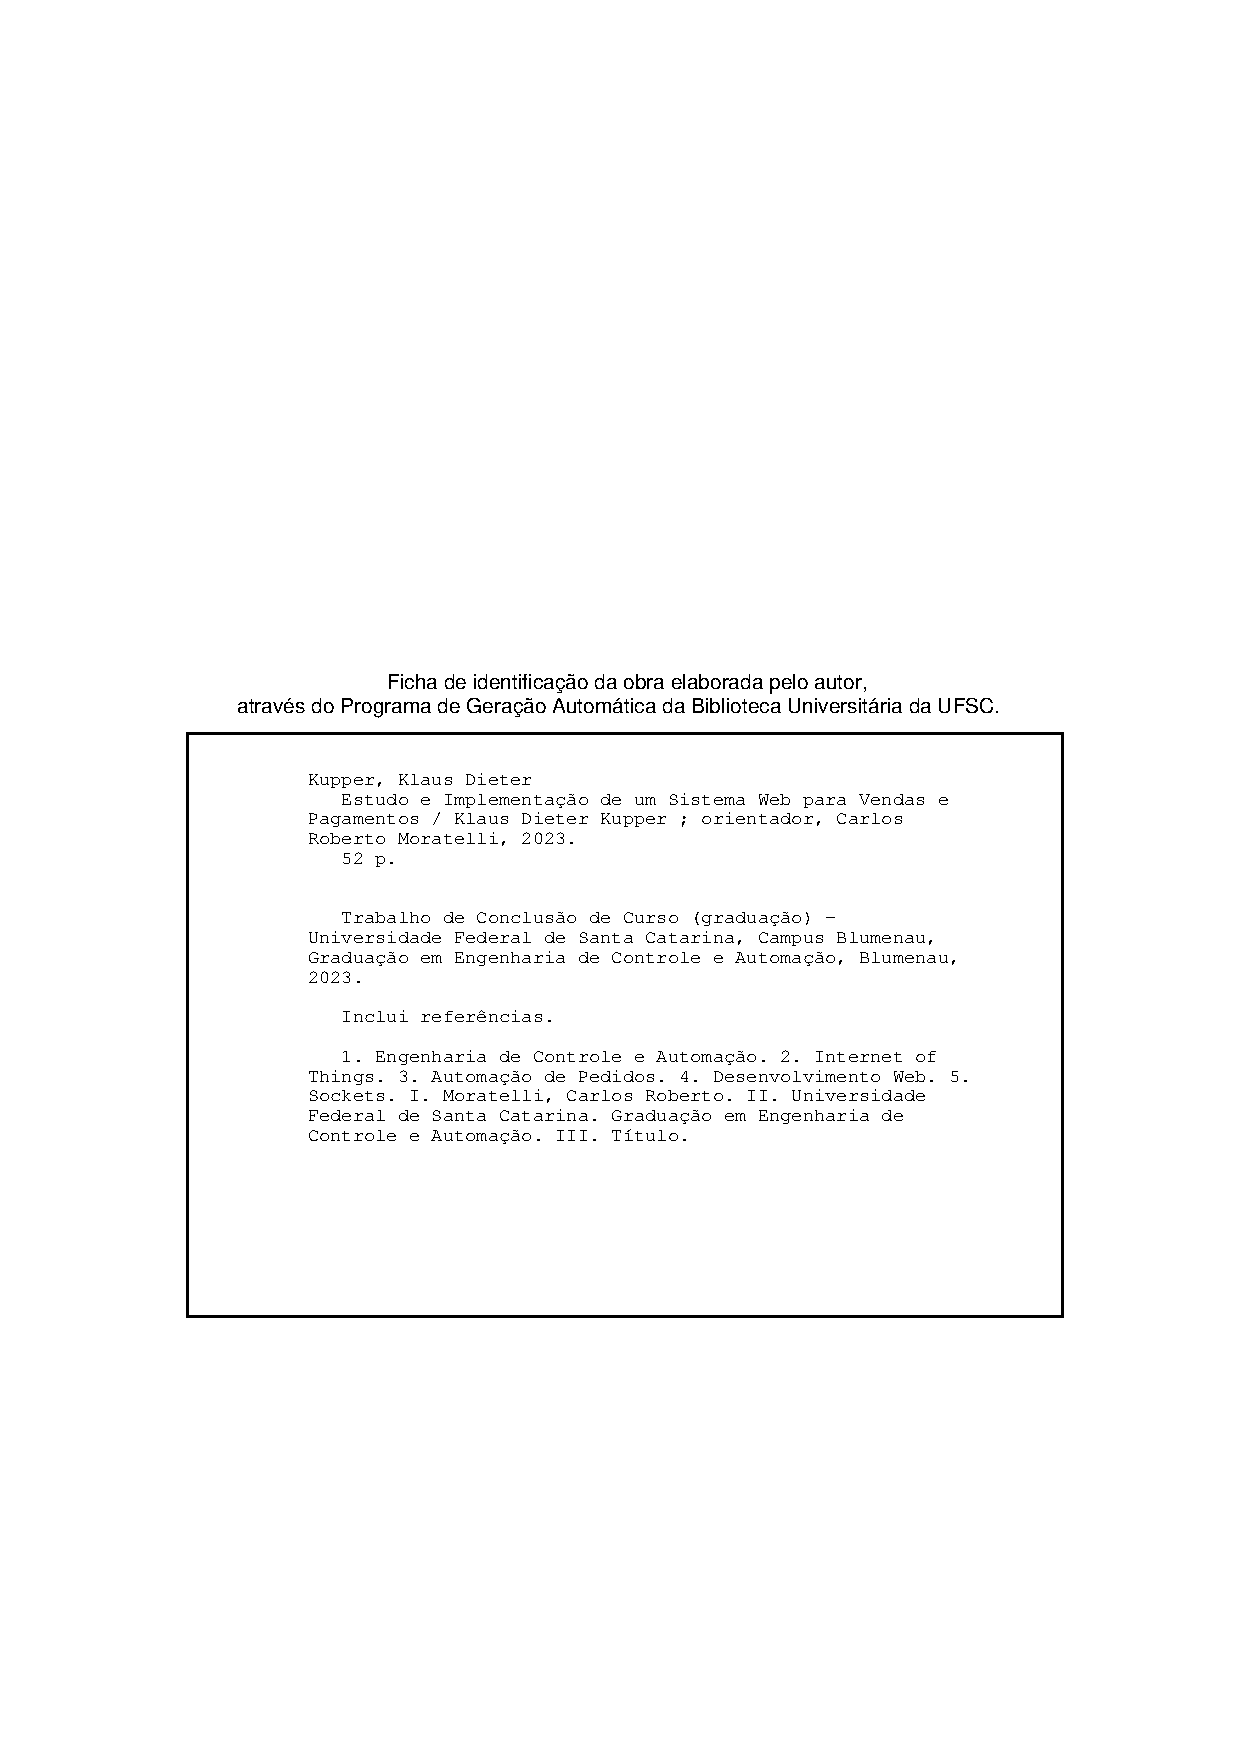
\includepdf{pre_textual/ficha_catalografica.pdf}
\end{fichacatalografica}

% Inserir folha de aprovação
\begin{folhadeaprovacao}
	\OnehalfSpacing
	\centering
	\imprimirautor\\%
	\vspace{24pt}		
	\textbf{\imprimirtitulo}%
	\ifnotempty{\imprimirsubtitulo}{:~\imprimirsubtitulo}\\%
	%		\vspace*{31.5pt}%3\baselineskip
	\vspace*{\baselineskip}
	%\begin{minipage}{\textwidth}
	Este Trabalho de Conclusão de Curso foi julgado adequado para obtenção do Título de ``\imprimirformacao'' e aprovado em sua forma final pelo Curso de Graduação em Engenharia de Controle e Automação.\\
	\vspace{12pt}
	\imprimirlocal, \imprimirdia~de~\imprimirmes~de~\imprimirano.\\
	
	\vspace*{18pt}
	\textbf{Banca Examinadora:}\\
	
	\vspace*{24pt}
	\assinatura{\OnehalfSpacing \imprimirbancaa}
	\vspace{6pt}
	Universidade Federal de Santa Catarina\\
	
	\vspace*{24pt}
	\assinatura{\OnehalfSpacing \imprimirbancab}
	\vspace{6pt}
	Universidade Federal de Santa Catarina\\
	
	\vspace*{24pt}
	\assinatura{\OnehalfSpacing \imprimirbancac}
	\vspace{6pt}
	Universidade Federal de Santa Catarina\\
	
\end{folhadeaprovacao}

% Dedicatória
\ifnotempty{\imprimirdedicatoriatcc}{
\begin{dedicatoria}
	\vspace*{\fill}
	\noindent
	\begin{adjustwidth*}{}{5.5cm} 
		\raggedleft       
		\imprimirdedicatoriatcc
	\end{adjustwidth*}
\end{dedicatoria}
}

% Agradecimentos
\ifnotempty{\imprimiragradecimentostcc}{
\begin{agradecimentos}
	\imprimiragradecimentostcc
\end{agradecimentos}
}

% Epígrafe
\ifnotempty{\imprimirepigrafetcc}{
\begin{epigrafe}
	\vspace*{\fill}
	\imprimirepigrafetcc
\end{epigrafe}
}


% Resumo
\setlength{\absparsep}{18pt} % ajusta o espaçamento dos parágrafos do resumo
\begin{resumo}
	\SingleSpacing
	\imprimirresumotcc
	
	\textbf{Palavras-chave}: \imprimirpalavraschave
\end{resumo}

% Abstract
\begin{resumo}[Abstract]
	\SingleSpacing
	\imprimirabstracttcc
		
	\textbf{Keywords}: \imprimirkeywords
\end{resumo}


{%hidelinks
	\hypersetup{hidelinks}
	
	% inserir lista de figuras
	\pdfbookmark[0]{\listfigurename}{lof}
	\listoffigures*
	\cleardoublepage

        % inserir lista de tabelas
	\pdfbookmark[0]{\listtablename}{lot}
	\listoftables*
	\cleardoublepage
 
	% inserir lista de abreviaturas e siglas (devem ser declarados no preambulo)
	\ifnotempty{\verificasiglas}{
	\imprimirlistadesiglas
	}
	
	% inserir o sumario
	\pdfbookmark[0]{\contentsname}{toc}
	\tableofcontents*
	\cleardoublepage
	
}%hidelinks

	% Elementos textuais
	\textual
	
	% 1 - Introdução
	% ----------------------------------------------------------
\chapter{Introdução} \label{cap:intro}
% ----------------------------------------------------------
% Motivation for environmental monitoring
% AI Increases the need for data, which can be supplied from sensors etc.
% Importance of Wireless Sensor Networks (WSNs) in environmental monitoring.
% Increasing relevance of low-power, long-range technologies like LoRa.
% Categorization: Water, Soil, and Air/Chemical monitoring.
% Smart cities?
% Outline of paper structure.


Floods, particularly flash floods, are among the most impactful natural disasters worldwide, causing substantial economic losses, infrastructure damage, and fatalities \cite{jonkman_2005_global, santos_2014_indstria}. These events are characterized by their sudden onset and rapid development, often occurring at the outlet of small catchments in response to intense localized rainfall, with response times of only a few hours \cite{borga_2014_hydrogeomorphic} . Compounding the issue, climate change is intensifying the global hydrological cycle, leading to an increase in the frequency and severity of extreme weather events, including floods. This reinforces the need for improved flood monitoring, risk management strategies and alert systems to safeguard communities \cite{hall_2014_understanding, bragana_2024_anlise}.

Flash floods and debris flows often escape conventional hydrometeorological monitoring due to their spatial and temporal unpredictability \cite{borga_2014_hydrogeomorphic,hall_2014_understanding}. Accurate and real-time data collection becomes essential to calibrate hydrological and hydrodynamic models such as rainfall–runoff systems, flood discharge and water supply volumes which serve as the foundation for effective early warning systems \cite{lin_2020_semantic, lo_2015_visual, iqbal_2021_how}. In addition to instrumental data, combining systematic flood observations with historical and documentary records has been highlighted as a valuable approach to better understand long-term flood regime dynamics, including the detection of flood-rich and flood-poor periods influenced by natural variability \cite{borga_2014_hydrogeomorphic,hall_2014_understanding,iqbal_2021_how, bragana_2024_anlise}.

However, monitoring natural disasters presents substantial technical challenges. The vast scales involved, coupled with harsh environmental conditions and the need for real-time data, demand robust, cost-effective, and scalable technological solutions. In this context, Wireless Sensor Networks (WSNs) have emerged as a promising tool, offering significant advantages in terms of deployment flexibility, rapid response capabilities, and affordability compared to traditional monitoring infrastructures. WSNs enable dense spatial sampling and continuous data collection, which are critical for disaster monitoring applications.\cite{chen_2013_natural, ferreira_2023_conception, pule_2017_wireless}

To further enhance WSN capabilities in remote and large-scale environments, Low Power Wide Area Networks (LPWAN) like LoRaWAN have gained prominence. LoRaWAN is specifically designed for transmitting small amounts of data over long distances with extremely low power consumption, enabling sensor nodes to operate autonomously for up to 10 years . This makes it particularly suitable for hydrological monitoring systems in regions with limited infrastructure \cite{pule_2017_wireless, chen_2013_natural,ferreira_2023_conception}. 

This Master's project aims to develop a WSN for river water level monitoring using LoRa technology, focusing on the performance comparison of low-cost LiDAR and ultrasonic sensors. The project will involve designing and implementing a microcontroller-based sensor node capable of interfacing with various sensors, including TF-Luna, TF-Nova, JSN-SR04T, and HC-SR04.

\section{Objectives}

The primary objective of this Master's project is to design, implement, and rigorously evaluate a LoRa-based WSN for river water level monitoring, focusing on a comprehensive performance comparison of selected low-cost LiDAR and ultrasonic sensors.

\section{Specific Objectives}

\begin{enumerate}
    \item To develop a microcontroller-based sensor node capable of interfacing with TF-Luna, TF-Nova, JSN-SR04T, and HC-SR04 sensors;
    \item To implement robust firmware for synchronized data acquisition, local data processing, and efficient LoRa/LoRaWAN data transmission.
    \item To conduct laboratory experiments to quantify and compare the accuracy, precision, range, resolution, and susceptibility to common interferences (e.g., temperature shifts, target surface variations, water conditions) of each sensor;
    \item To deploy the developed sensor nodes in a real environment, assessing their performance, data integrity, and operational resilience against ambient environmental conditions;
    \item To analyze the collected field and lab data to provide a assessment of the sensors, identifying their respective strengths, weaknesses, and optimal operational conditions for river stage monitoring;
    \item To offer evidence-based recommendations for sensor selection, node design, and LoRa network deployment strategies for scalable and cost-effective hydrological monitoring systems in similar regional contexts;
\end{enumerate}

\section{Structure of the Work}

This thesis is structured as follows:
\begin{itemize}
    \item \textbf{Chapter 2: Literature Review} - A comprehensive review of existing literature on WSNs, LoRa technology, and sensor technologies for hydrological monitoring.
    \item \textbf{Chapter 3: Materials and Methods} - Detailed description of the hardware and software design, sensor selection criteria, experimental setup, and data analysis methods.
    \item \textbf{Chapter 4: Laboratory Experiments} - Presentation and analysis of laboratory results comparing the selected sensors under controlled conditions.
    \item \textbf{Chapter 5: Field Deployment} - Description of the field deployment process, network setup, and performance evaluation in a real riverine environment.
    \item \textbf{Chapter 6: Discussion and Conclusion} - Summary of findings, implications for future research, and recommendations for practical applications in water level monitoring.
\end{itemize}



	
	% 2 - Desenvolvimento
	\chapter{Literature Review}

% 2 Sensors and Technologies for Environmental Monitoring
% Sensor classification from that “sensors daily use…” - Active or passive and applications.
% 2.1 Water Monitoring
% Focus: Water level (ultrasonic, LiDAR, float sensors),Water quality (pH, turbidity, EC sensors), flood detection, river monitoring.
% Innovations: Archimedes-based sensors, object recognition methods, SAW?.

% Relevant Articles:
% 1"An Intelligent Water Level Estimation System" — Uses object recognition via deep learning for water levels. (Observations: Estimation via camera + ML.)
% 2"A Technical Evaluation of Lidar-Based Measurement of River Water Levels" — Discusses LiDAR for precise water monitoring. (High relevance.)
% 3"A low-cost ultrasonic sensor for online monitoring of liquid level" — Simple ultrasonic-based approach. (Low relevance but practical example.)
% 4"SAW Sensor based a Novel Hydrostatic Liquid Level Sensor" — Novel SAW-based liquid level sensor. (Observation: Hydrostatic pressure with SAW.)
% 5"Modeling and testing of a highly sensitive surface acoustic wave hydrostatic liquid level sensor" — Focus on SAW tech for water levels.
% 6"Development of liquid level measurement technologies: A review" — Industrial-focused review of level sensors.


% 2.2 Soil Monitoring
% Focus: Soil moisture, nutrients, agriculture precision.
% Use of SAW sensors, RFID-based systems, and nanotechnology.
% Relevant Articles:
% 1"Smart Agriculture Systems: Soil Sensors and Plant Wearables for Smart and Precision Agriculture" — Extensive review, strong base for soil monitoring section. (MIT paper, highly relevant.)
% 2"Conception and Design of WSN Sensor Nodes Based on Soil Moisture Monitoring" — Focus on soil pH, turbidity, and temperature sensors. (Observation: Detailed sensor design.)
% 3"Applications of Sensor Networks and Remote Sensing in Precision Agriculture" — General but with some relevance to WSN in agriculture. (Observation: Somewhat shallow but covers multiple angles.)

% 2.3 Air and Chemical Monitoring
% Focus: Air quality, gas detection, environmental chemical monitoring.
% "SAW Sensors for Chemical Vapors and Gases" — Discusses SAW sensor principles for air/gas detection. (Observation: Emphasizes SAW advantages like sensitivity and robustness.)
% "A Progress Review on Solid‐State LiDAR and Nanophotonic Sensors" — Discusses LiDAR, photonic sensors applicable to particulate air detection or similar use cases.

This study proposes the development of a water level monitoring system using LoRa-based WSNs and evaluating different non-contact measurement methods. The choice for a wireless and non-contact reading sensor node is the most recommended in the sensing application of unhealthy and harsh environments because it has independent processing and wireless signal transmission. They have a significant advantage over traditional wired sensors, which are not a cheap and viable option for this type of application \cite{bhuyan_2010_intelligent}.



--------- General LORA REVIEW MENTIONS ------  GENERAL FLOOD REVIEW MENTIONS ------ ?? maybe put on fundaments chapter

Previously ultrasonic was defined as viable option to monitor water levels in river and channels using the sensor model GY-Us42, with results indicating that the device's average error is below 3\% \cite{mohammadrezamasoudimoghaddam_2024_a}. Other work concludes that the ultrasonic sensor model HC-SR04 is a technically and economically viable alternative to monitor water levels \cite{ pereira_2022_evaluation}, and the same sensor model is also praised as a good option for education, citizen science, and research due to low cost \cite{bresnahan_2023_a}. 

In previous research, LiDAR was explored as a cost-effective sensor for measuring water leves from bridges, with lab and field tests indication a good accuracy with 0.1\% error, but significant variations caused by sensor temperature and water roughness \cite{paul_2020_a}. LiDAR sensors installed on river banks for flash flood monitoring were also tested with good results, and indication that different amounts of small suspended particles on water could impact the results, and that the sensor could also be used to monitor these suspended particles \cite{tamari_2016_flash}. Another study explored how the LiDAR sensor model TF-mini compared to linigraph pressure sensors, showing the benefits of a non-contact measurement method of the LiDAR compared to a contact one with the linigraph and validating the LiDAR as an excellent choice among fluid level measurement technologies compared \cite{santana_2024_development}.

The contribution of this work is exploring more of the two different methods of non-contact water level measurement, comparing and definig best applications for each one. Adding to it, this work will also explore creating a low-cost, low-power, and long-range water level monitoring system using LoRaWAN technology. The system will be designed to operate in challenging environments, such as flood-prone river systems, where other more traditional monitoring methods may be impractical or too expensive.

	
	% 3 - Seção
	\chapter{Theoretical Framework} \label{cap:theoretical}

% 3. Wireless Sensor Networks (WSN) and Communication Technologies
% Focus on how WSN enables data collection, data transmission, and real-time monitoring.
% Discussion on technologies like LoRa, LPWAN, Zigbee, bt, web.
% LoRa and LPWAN dominance in environmental WSN
% Architectures? Mesh vs. star topologies. Use of gateways, cloud services, and edge computing nodes etc

% Relevant Articles:
% "Long Battery Life IoT Sensing by Beat Sensors" — Communication based on timing intervals. (Observation: Alternative low-power communication model.)
% "Exploiting hardware vulnerabilities to attack embedded system devices" — Security challenges in WSN. (Observation: Survey of microarchitectural attacks.)
% "Conception and Design of WSN Sensor Nodes Based on Soil Moisture Monitoring" — Also relevant here for its WSN node design discussion.

% "LoRa provided reliable communication over 5km in rural tests."
% "Battery life extended to 5 years using beat sensors."
% Mention the use of AI/ML for sensor data analysis, anomaly detection, or pattern recognition. Some articles on water monitoring use CNN-based object detection for water level estimation.


This chapter presents the theoretical foundation underpinning the development of the proposed water level monitoring system. It discusses the essential technologies and concepts, including the \glsxtrfull{IoT}, long-range wireless communication (\glsxtrfull{LoRa}/\gls{LoRaWAN}), distance measurement methods such as \glsxtrfull{LiDAR} and ultrasonic sensors, and embedded systems. These topics establish the context and technical justification for the architecture adopted in this work.

\section{\glsxtrfull{IoT}}

The \gls{IoT} encompasses a network of interconnected physical objects that are equipped with sensors, processors, and communication interfaces, allowing them to collect, process, and transmit data without human intervention . The proliferation of \gls{IoT} has enabled the deployment of intelligent systems in areas such as agriculture, industrial monitoring, and environmental surveillance. \cite{Madakam:2015,javaid_2021_sensors}

In this project, \gls{IoT} concepts are applied to create an autonomous and distributed sensor network capable of collecting hydrological data and transmitting it remotely for analysis and visualization. The figure \ref{fig:iot} illustrates how various devices connect to the internet through \gls{IoT}, enabling data exchange and interaction between the physical and digital worlds. \cite{javaid_2021_sensors}

\begin{figure}[h]
    \centering
    \caption{Internet of Things.}
    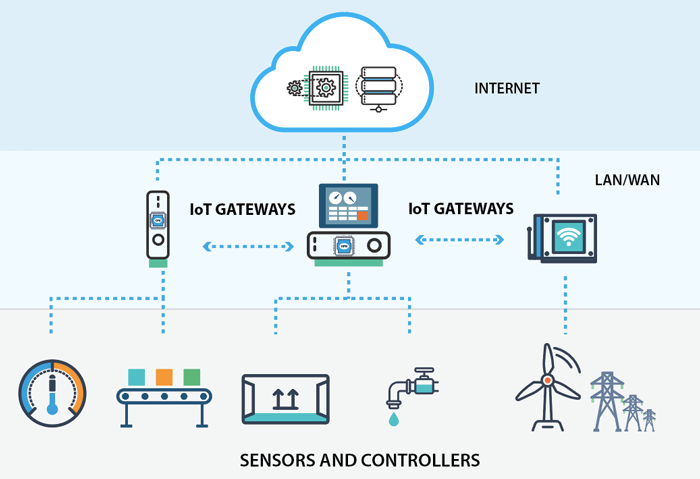
\includegraphics[width=0.8\textwidth]{figuras/iot.png}
    \fonte{\cite{iot123}.}
    \label{fig:iot}
\end{figure}

\section{LoRa and LoRaWAN}

\glsxtrfull{LoRa} is a proprietary spread spectrum modulation technique on the basis of \glsxtrfull{CSS}, which is resilient and robust against interference and noise, it also provides a solution for long-range and ultra-low power-consumption transmission, using unlicensed radio bands such as 868 MHz (Europe) and 915 MHz (Americas) \cite{sun_2022_recent}.

\glsxtrfull{LoRaWAN} is the \glsxtrfull{MAC} protocol built on top of \gls{LoRa}, specifying how end-devices communicate with central gateways and application servers,  defining a typical star-topology network architecture and its bi-directional communication protocol. The technology has been designed for applications that need to send small amounts of data over long distances a few times per day. Its low power features offers the capability to achieve autonomy of up to 10 years. \cite{pule_2017_wireless,sun_2022_recent}. Such long-range and energy-efficient communication demands have inspired the emergence of Low Power Wide Area Networks (LPWANs) as a new \gls{IoT} paradigm, which fills the gap of legacy wireless communication technologies shown in Figure \ref{fig:lora}. 

\begin{figure}[h]
    \centering
    \caption{Comparison with legacy wireless communication technologies.}
    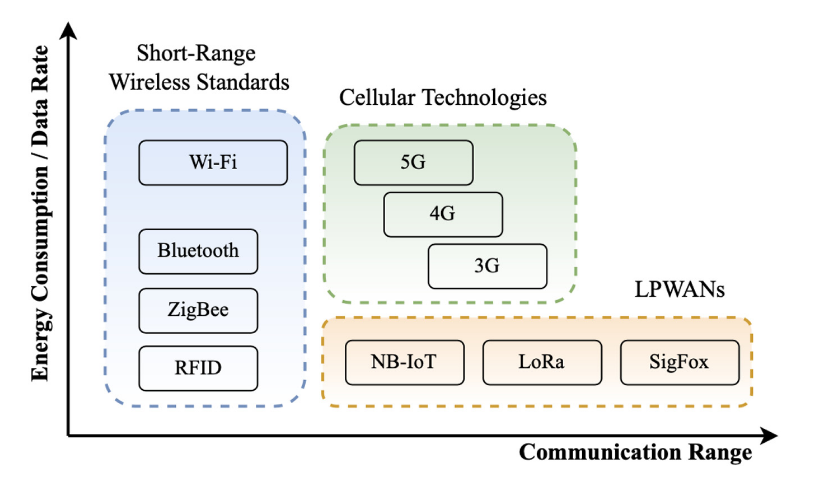
\includegraphics[width=0.8\textwidth]{figuras/Lora-comparison.png}
    \fonte{\cite{sun_2022_recent}.}
    \label{fig:lora}
\end{figure}

\section{Microcontroller ESP8266}

Embedded systems are specialized computing systems designed to perform dedicated functions within larger systems, often under real-time constraints. The NodeMCU ESP8266 is a microcontroller based on the ESP8266 platform, which features integrated Wi-Fi connectivity. It is widely used in \gls{IoT} projects due to its ease of programming, low cost, and advanced features. The ESP8266, shown in Figure \ref{fig:node}, is particularly suitable for such applications due to its ability to operate at low power, which is crucial for battery-powered devices, and its capability to connect to Wi-Fi networks, enabling communication with the internet and other devices on the network \cite{Kolban2016}.\cite{datasheet_2023_esp8266ex}

\begin{figure}[h]
    \centering
    \caption{ESP8266 NodeMcu.}
    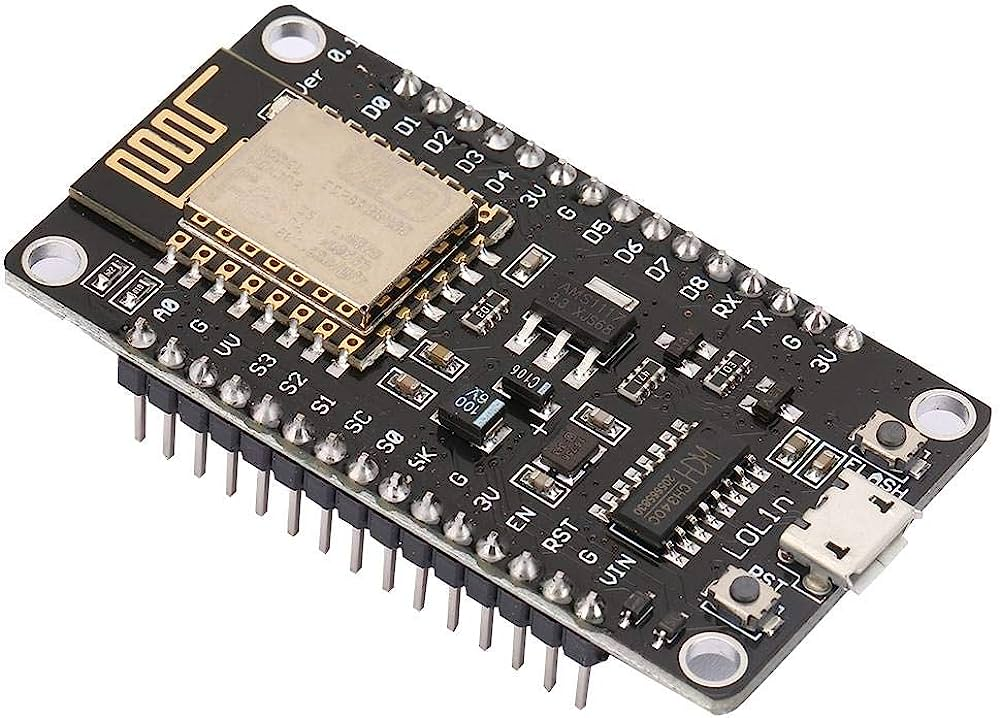
\includegraphics[width=0.5\textwidth]{figuras/nodemcu.jpg}
    \fonte{\cite{nodemcu}.}
    \label{fig:node}
\end{figure}

\section{LiDAR}

\glsxtrfull{LiDAR} technology enables the accurate determination of an object's distance (and velocity) information. LiDAR technology is widely used in metrology, environment monitoring, archaeology, and robotics. Compared with more mature \glsxtrfull{RADAR} technology, LiDAR makes use of optical wave, which is at shorter wavelength regime compared with radio wave, and hence has potential to achieve higher precision in 3D sensing.\cite{li_2022_a, lednev_2013_remote,behroozpour_2017_lidar,javaid_2021_sensors}.

The principle of lidar ranging relies on the rugosity of the reflective surface to generate nonspecular reflection (i.e., scattering) of the incipient laser beam. As with radar, lidar ranging measures time of flight, but it uses higher frequency waves for greater pulse intensities. Near-infrared (NIR) light is most commonly used for this purpose, typically over wavelengths of 900–1,100 nm (270–330 THz) due to the low cost of lasers operating in this wavelength range and lower energy density than the visible spectrum.\cite{li_2022_a, fernandezdiaz_2014_early, smart_2009_river, behroozpour_2017_lidar}. The laser wavelength is a critical factor in determining the sensor's performance, as it influences the interaction with water and suspended particles. Figure \ref{fig:laser-wavelength-graphs} illustrates the spectral character of clear still water as a function of laser wavelength and the influence of suspended sediment concentration on reflectance in rivers \cite{lednev_2013_remote,milan_2010_mapping,paul_2020_a}.

\begin{figure}[h]
    \centering
    \caption{(a) Spectral character of clear still water as a function of laser wavelength \cite{lednev_2013_remote,milan_2010_mapping}. (b) Influence of suspended sediment concentration (curves: units of mg L(-1)) in river upon reflectance \cite{paul_2020_a, milan_2010_mapping}}
    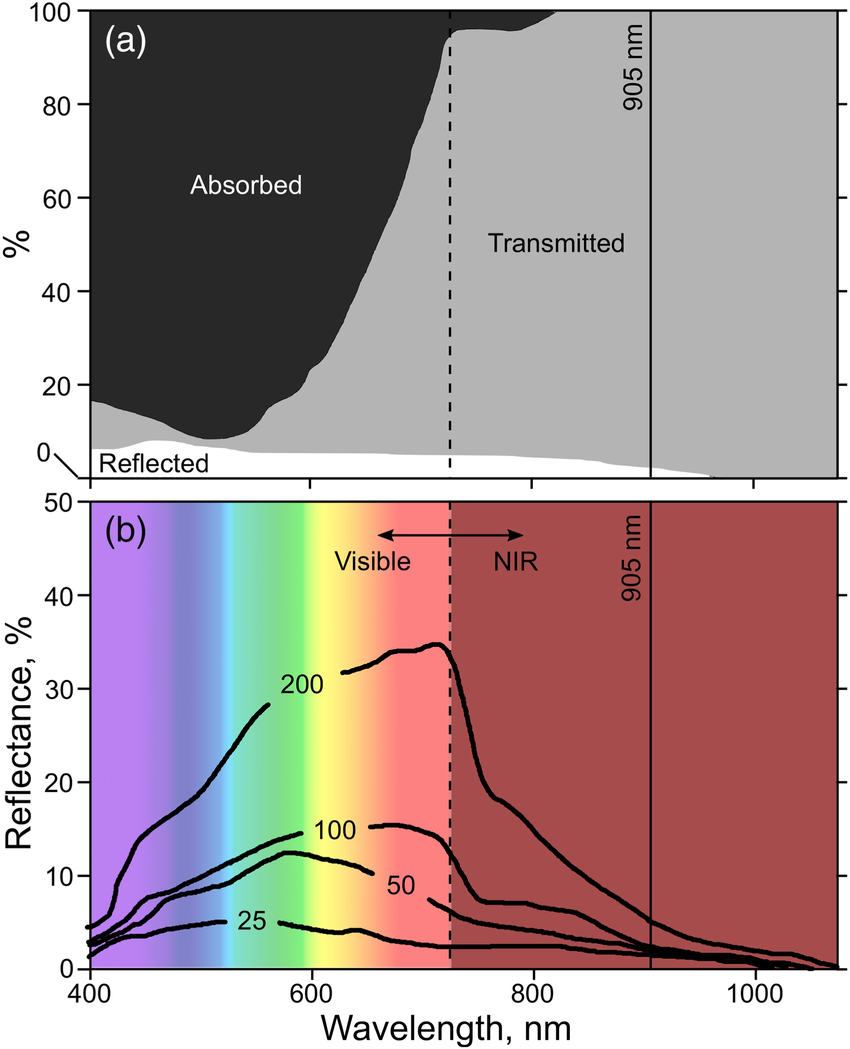
\includegraphics[width=0.8\textwidth]{figuras/light-absorption.png}
    \fonte{\cite{lednev_2013_remote,milan_2010_mapping,paul_2020_a}.}
    \label{fig:laser-wavelength-graphs}
\end{figure}

The three sensing schemes most commonly used in LiDAR sensors are: pulsed \glsxtrfull{TOF}, AMCW \gls{TOF}, and FMCW. \cite{li_2022_a,behroozpour_2017_lidar}. For this work the most important ones are the pulsed \gls{TOF} and AMCW \gls{TOF}, which are described below.

\subsection{Pulsed Time of Flight (TOF)}
The pulsed TOF LiDAR works based on the time delay of an optical pulse emitted by the TX, reflected from the sensing object, and received by the RX. The sensing distance can be expressed using the following equation \cite{li_2022_a}.

\begin{equation}
    d = \frac{c \cdot \Delta t}{2}
\end{equation}

where \(d\) is the distance to the object in meters, \(c\) is the speed of light, and \( \Delta t\) is the time delay between emission and reception of the optical pulse in seconds.

\subsection{Amplitude Modulated Continuous Wave (AMCW) Time of Flight (TOF)}
AMCW TOF LiDAR uses a continuous wave laser that is modulated in amplitude. The phase difference between the transmitted and received signals is measured to determine the distance to the object. The distance can be calculated using the following equation \cite{li_2022_a}.

\begin{equation}
    d = \frac{c \cdot \Delta \phi}{4\pi f}
\end{equation}

where \(d\) is the distance to the object in meters, \(c\) is the speed of light, \(\Delta \phi\) is the phase difference between the transmitted and received signals, and \(f\) is the modulation frequency in Hz.

\section{Ultrasonic Sensors}

Ultrasonic sensors estimate distance by transmitting high-frequency acoustic waves and measuring the echo delay. Common models like the HC-SR04 and JSN-SR04T are widely used in academic and industrial applications due to their low cost and simplicity \cite{bresnahan_2023_a,akhileshnagpure_2022_water,mohammadrezamasoudimoghaddam_2024_a}.

The basic principle of ultrasonic distance measurement is based on the time of flight (\gls{TOF}) of sound waves. The sensor emits a high-frequency sound wave, which travels through the air, reflects off an object, and returns to the sensor.

\section{Wireless Sensor Network (WSN)}

\glsxtrfull{WSN} are considered a promising alternative to complement conventional monitoring processes. These networks are relatively affordable and allow measurements to be taken remotely, in real-time and with minimal human intervention \cite{pule_2017_wireless}. A \gls{WSN} is composed of spatially distributed autonomous nodes that monitor physical or environmental conditions. These nodes typically consist of a sensing unit, processing unit, communication interface, and power source. Natural disaster monitoring is very complex and imposes a number of challenges mainly due to huge scales,uncertainties, and harsh environments.

Each such sensor network node typically has many parts: a radio transceiver with an internal antenna or connection to an external antenna, a microcontroller, an electronic circuit for interfacing with the sensors and an energy source, usually a battery or an embedded form of energy harvesting \cite{yellampalli_2021_wireless}. An example architecture of a WSN is shown in Figure \ref{fig:wsn-graphs}. The nodes are capable of collecting data from the environment, processing it, and transmitting it wirelessly to a base station or gateway for further analysis and visualization. A \gls{WSN} can be single hop, where the nodes connect directly to the base station, or multi-hop, where the nodes can send information between themselves before reaching the base station \cite{yellampalli_2021_wireless}.

\begin{figure}[h]
    \centering
    \caption{Wireless Sensor Network architecture.}
    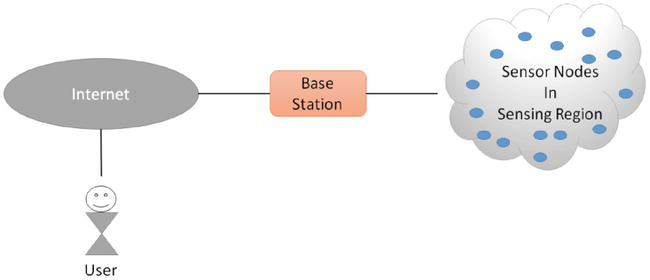
\includegraphics[width=0.8\textwidth]{figuras/WSN_architecture.png}
    \fonte{\cite{yellampalli_2021_wireless}.}
    \label{fig:wsn-graphs}
\end{figure}

WSN-based natural disaster monitoring systems excel in terms of cost, speed of response, scalability and flexibility in contrast to conventional approaches. In general, disaster monitoring with WSN manifests a typical paradigm of data-intensive application upon low-cost scalable system \cite{chen_2013_natural, pule_2017_wireless, ferreira_2023_conception}. In this work, the \gls{WSN} architecture facilitates distributed hydrological data collection and centralized data aggregation through \gls{LoRa} communication.

\section{Time-Series Data and Environmental Monitoring}

Time-series data represent sequential observations over time. In the context of water level monitoring, time-series analysis enables the detection of trends, anomalies, and correlations between environmental factors \cite{lozano_2017_sensors}. Basic statistical techniques—such as moving averages, root mean square error (\glsxtrfull{RMSE}), and filtering—are applied to improve data reliability and reduce noise\cite{santana_2024_development}. 


	
	% 4 - Conclusão
	% ----------------------------------------------------------
\chapter{Conclusão}\label{cap:conclusao}
% ----------------------------------------------------------

A proposta deste projeto foi desenvolver um sistema para automação de pedido e compras em pontos de venda, que permita integração com agentes de distribuição, de forma a automatizar todo o processo.

Com base nos resultados apresentados, pode-se concluir que o desenvolvimento do sistema obteve sucesso. A aplicação web desenvolvida permite que os usuários possam fazer seus pedidos, enquanto os funcionários dos pontos de venda têm acesso a informações precisas sobre os pedidos realizados, podendo acompanhar o status da entrega em tempo real. Além disso, o servidor de \textit{sockets} permite que os pontos de venda possam notificar os agentes de distribuição de qualquer atualização no status dos pedidos, de forma rápida e eficiente.

Por fim, a utilização de serviços de hospedagem em nuvem garantiu a disponibilidade e a escalabilidade do sistema, permitindo que ele possa ser usado por um grande número de usuários ao mesmo tempo.

Dessa forma, pode-se afirmar que o sistema de gerenciamento de pedidos para pontos de venda desenvolvido neste trabalho é uma solução eficiente e viável para empresas que desejam aprimorar seus processos de gerenciamento de pedidos e melhorar a experiência dos seus clientes, usando automação e tecnologias web modernas.

Para trabalhos futuros deseja-se incluir melhorias na interface, principalmente para exibir mais informações sobre os pedidos, e de forma geral torna-la mais amigável. Além disso, outro ponto que pode ser trabalhado seria o desenvolvimento de agentes de distribuição, conectando o NodeMCU com uma máquina de café, por exemplo, e distribuindo realmente os produtos.
	
	
	% Elementos pós-textuais
	\postextual
	
	
	% Referências bibliográficas
	\begingroup
	    \printbibliography[title=REFERÊNCIAS]
	\endgroup
	
	
	%Reconfiguração do título para apêndices e anexos
	 \renewcommand{\ABNTEXchapterupperifneeded}[1]{#1} 
	\makeatletter
	\settocpreprocessor{chapter}{%
      \let\tempf@rtoc\f@rtoc%
      \def\f@rtoc{%
      \texorpdfstring{{\tempf@rtoc}}{\tempf@rtoc}}%
      }
    \makeatother
	
	
	% Apêndices
    %\begin{apendicesenv}
    	%\partapendices* 
    	%% ----------------------------------------------------------
\chapter{Descrição}   %Apenas a primeira letra deve ser maiúscula
% ----------------------------------------------------------

Textos elaborados pelo autor, a fim de completar a sua argumentação. Deve ser precedido da palavra APÊNDICE, identificada por letras maiúsculas consecutivas, travessão e pelo respectivo título. Utilizam-se letras maiúsculas dobradas quando esgotadas as letras do alfabeto. 

    %\end{apendicesenv}

    % Anexos
    %\begin{anexosenv}
    	%\partanexos*
    	%% ----------------------------------------------------------
\chapter{Descrição}   %Apenas a primeira letra deve ser maiúscula
% ----------------------------------------------------------

São documentos não elaborados pelo autor que servem como fundamentação (mapas, leis, estatutos). Deve ser precedido da palavra ANEXO, identificada por letras maiúsculas consecutivas, travessão e pelo respectivo título. Utilizam-se letras maiúsculas dobradas quando esgotadas as letras do alfabeto. 

    %\end{anexosenv}

\end{document}